\documentclass[polish,a4paper]{article}
\usepackage{amsmath}
\usepackage{amssymb, amsfonts, amsthm, amsmath, bm}
\usepackage[T1]{fontenc}
\usepackage[utf8]{inputenc}
\usepackage{babel}
\usepackage{pslatex}
\usepackage{pgfplots}
\usepackage{hhline}
\usepackage[american]{circuitikz} 
\usepackage{anysize}
\usepackage{graphicx}
\DeclareGraphicsExtensions{.jpg}
\marginsize{2.5cm}{2.5cm}{3cm}{3cm}
\bibliographystyle{IEEEtran}


%makro do indeksów w tabeli
\newcommand{\PRzFieldDsc}[1]{\sffamily\bfseries\scriptsize #1}

%makro do informacji w tabeli
\newcommand{\PRzFieldCnt}[1]{\itshape #1}

%potężne makro tworzące tabelę z informacjami o teamie
\newcommand{\PRzHeading}[8]{
%% #1 - nazwa laboratorium
%% #2 - kierunek 
%% #3 - specjalność 
%% #4 - rok studiów 
%% #5 - symbol grupy lab.
%% #6 - temat 
%% #7 - numer lab.
%% #8 - skład grupy ćwiczeniowej

\begin{center}
\begin{tabular}{ p{0.32\textwidth} p{0.15\textwidth} p{0.15\textwidth} p{0.12\textwidth} p{0.12\textwidth} }

  &   &   &   &   \\
\hline
\multicolumn{5}{|c|}{}\\[-1ex]
\multicolumn{5}{|c|}{{\LARGE #1}}\\
\multicolumn{5}{|c|}{}\\[-1ex]

\hline
\multicolumn{1}{|l|}{\PRzFieldDsc{Kierunek}}	& \multicolumn{1}{|l|}{\PRzFieldDsc{Specjalność}}	& \multicolumn{1}{|l|}{\PRzFieldDsc{Rok studiów}}	& \multicolumn{2}{|l|}{\PRzFieldDsc{Symbol grupy lab.}} \\
\multicolumn{1}{|c|}{\PRzFieldCnt{#2}}		& \multicolumn{1}{|c|}{\PRzFieldCnt{#3}}		& \multicolumn{1}{|c|}{\PRzFieldCnt{#4}}		& \multicolumn{2}{|c|}{\PRzFieldCnt{#5}} \\

\hline
\multicolumn{4}{|l|}{\PRzFieldDsc{Temat Laboratorium}}		& \multicolumn{1}{|l|}{\PRzFieldDsc{Numer lab.}} \\
\multicolumn{4}{|c|}{\PRzFieldCnt{#6}}				& \multicolumn{1}{|c|}{\PRzFieldCnt{#7}} \\

\hline
\multicolumn{5}{|l|}{\PRzFieldDsc{Skład grupy ćwiczeniowej oraz numery indeksów}}\\
\multicolumn{5}{|c|}{\PRzFieldCnt{#8}}\\

\hline
\multicolumn{3}{|l|}{\PRzFieldDsc{Uwagi}}	& \multicolumn{2}{|l|}{\PRzFieldDsc{Ocena}} \\
\multicolumn{3}{|c|}{\PRzFieldCnt{\ }}		& \multicolumn{2}{|c|}{\PRzFieldCnt{\ }} \\

\hline
\end{tabular}
\end{center}
}
%koniec potężnego makro do tabeli

\begin{document}

%stworzenie tabeli - miejsce na zmienianie danych w tabeli
%indeksy do uzupełnienia
\PRzHeading{Laboratorium Podstaw Elektroniki}{Informatyka}{--}{I}{I1}{Układy wzmacniaczy operacyjnych}{6}{Ewa Fengler(132219), Sebastian Maciejewski(132275), Jan Techner(132332)}{}

%ZADANIA

\section*{Cel}
Celem przeprowadzanych doświadczeń jest poznanie funkcji wzmacniaczy operacyjnych w układach elektronicznych.

\section{Zadanie 1.3}

\subsection*{6.}
amplitudy
\subsection*{7.}
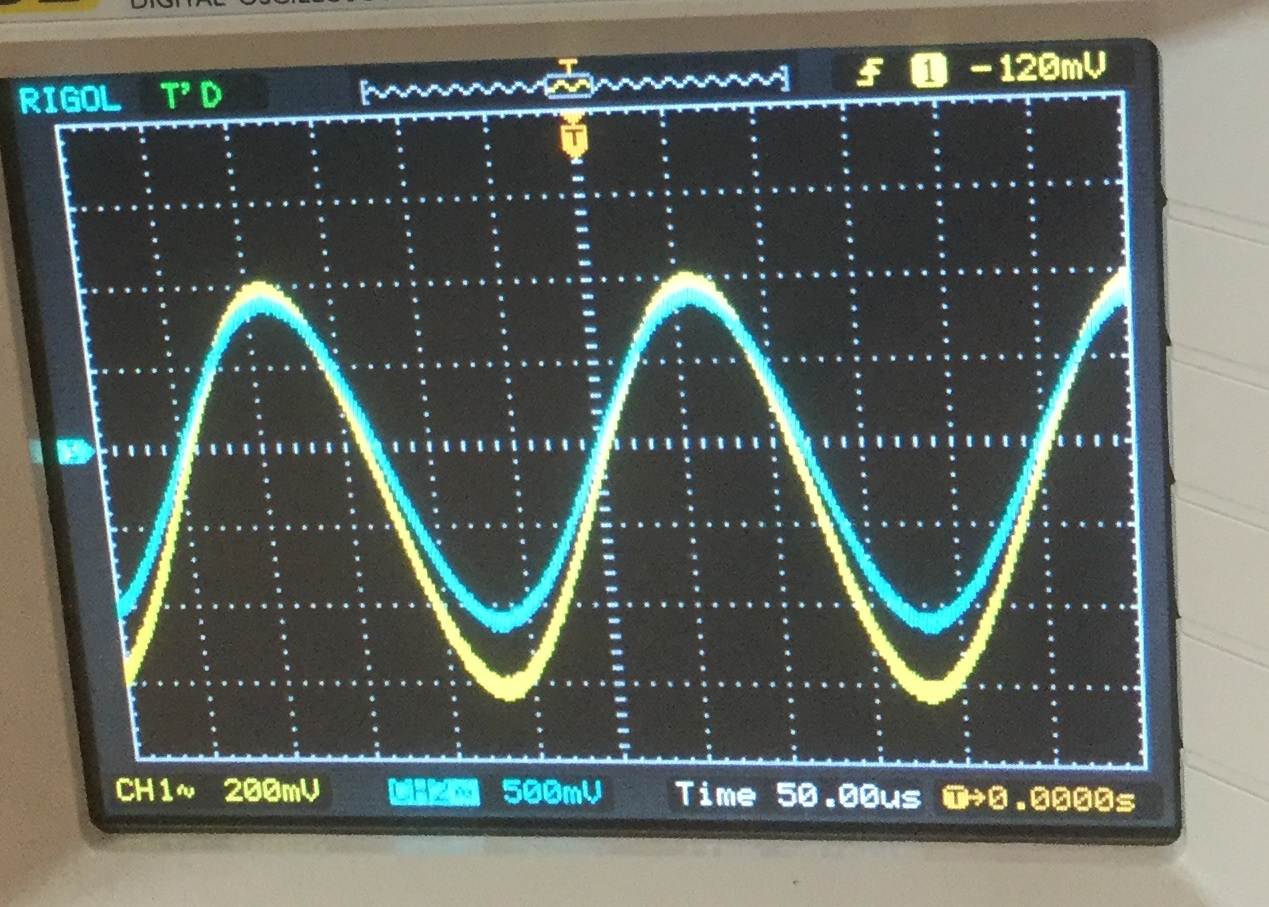
\includegraphics[scale=0.5]{amplituda}
\subsection*{8.}
oszacuj wzmocnienie
\subsection*{9.}
porównaj wzmocnienia
\subsection*{10.}
wnioski

\section{Zadanie 1.4}

\subsection*{1.}

\subsection*{4.}
tabelka
\subsection*{5.}
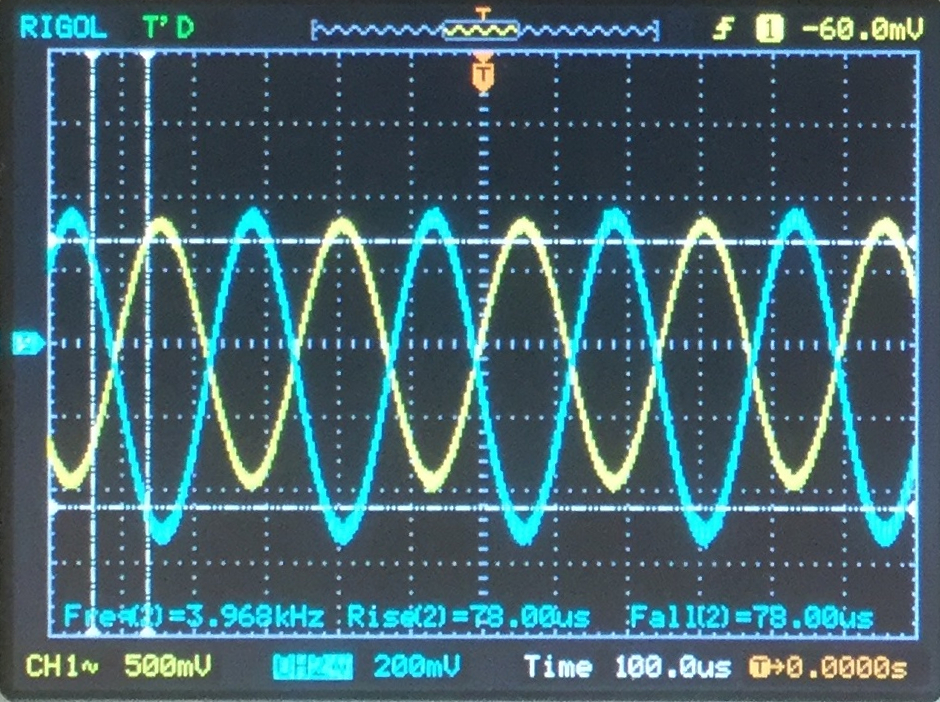
\includegraphics[scale=0.5]{czestotliwosc}
\subsection*{6.}
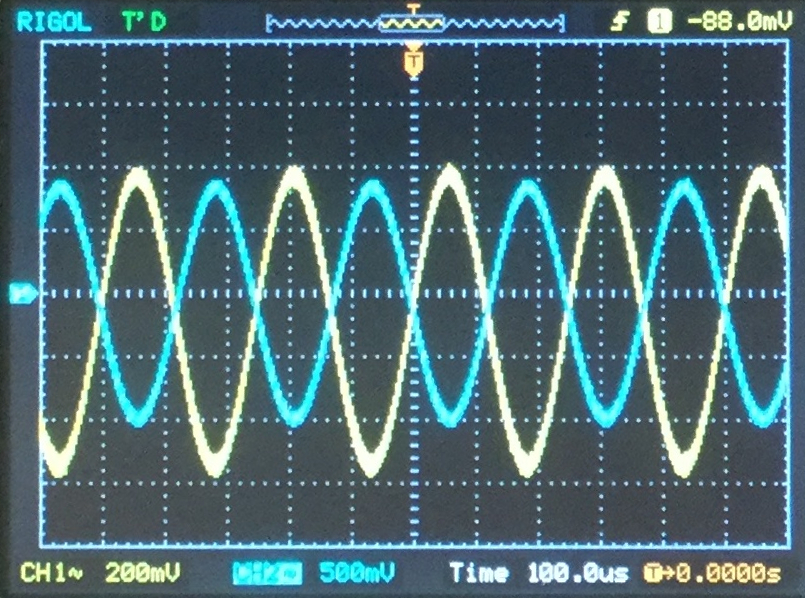
\includegraphics[scale=0.5]{k_odwracajaca}
\subsection*{7.}
komentarz
\subsection*{8.}
wnioski

\section{Zadanie 1.5}

\subsection*{1.}
schemat?
\subsection*{4.}
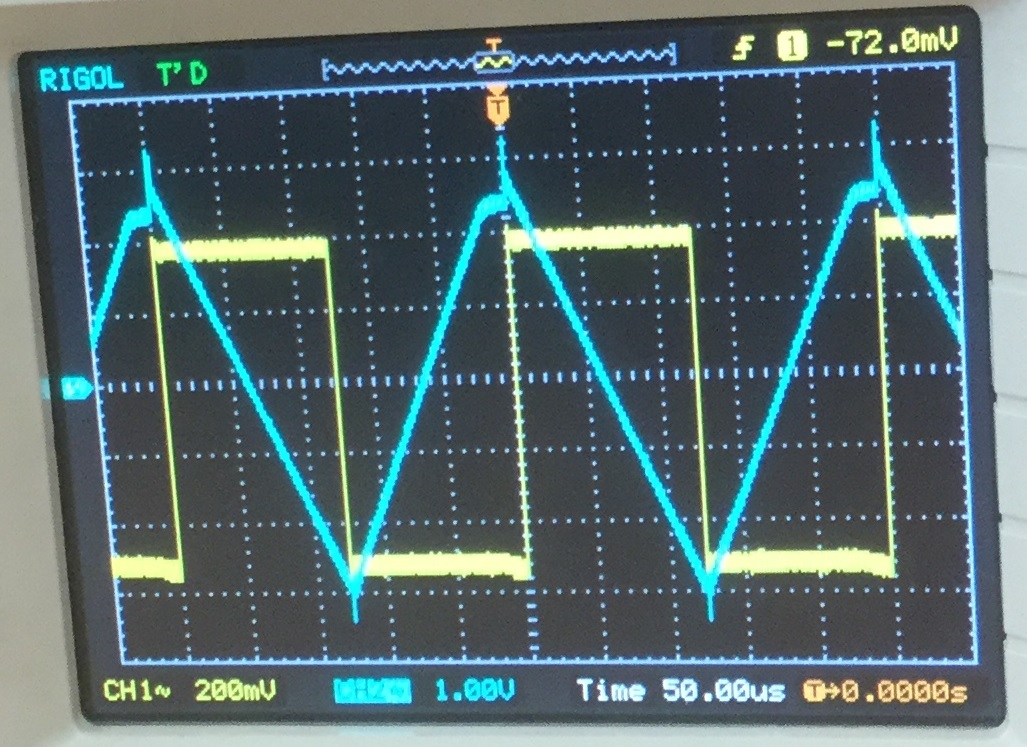
\includegraphics[scale=0.5]{przebieg_trojkatny}
\subsection*{5.}
zdjęcie i obliczenie nachylenia
1. Wiersz tabeli: 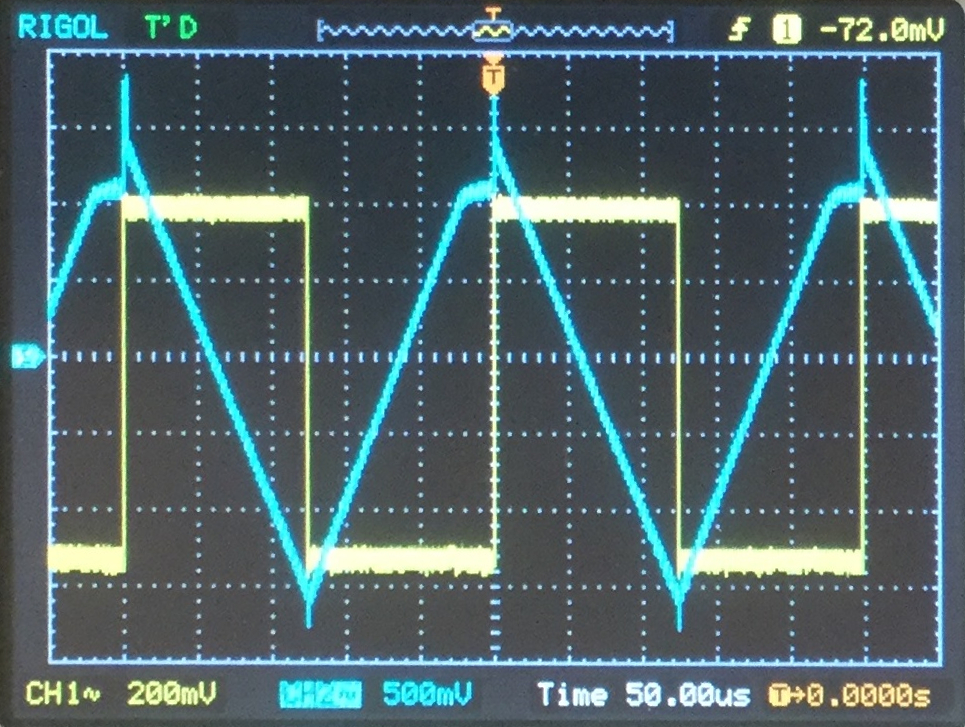
\includegraphics[scale=0.5]{r1c4}\\
2. Wiersz tabeli: 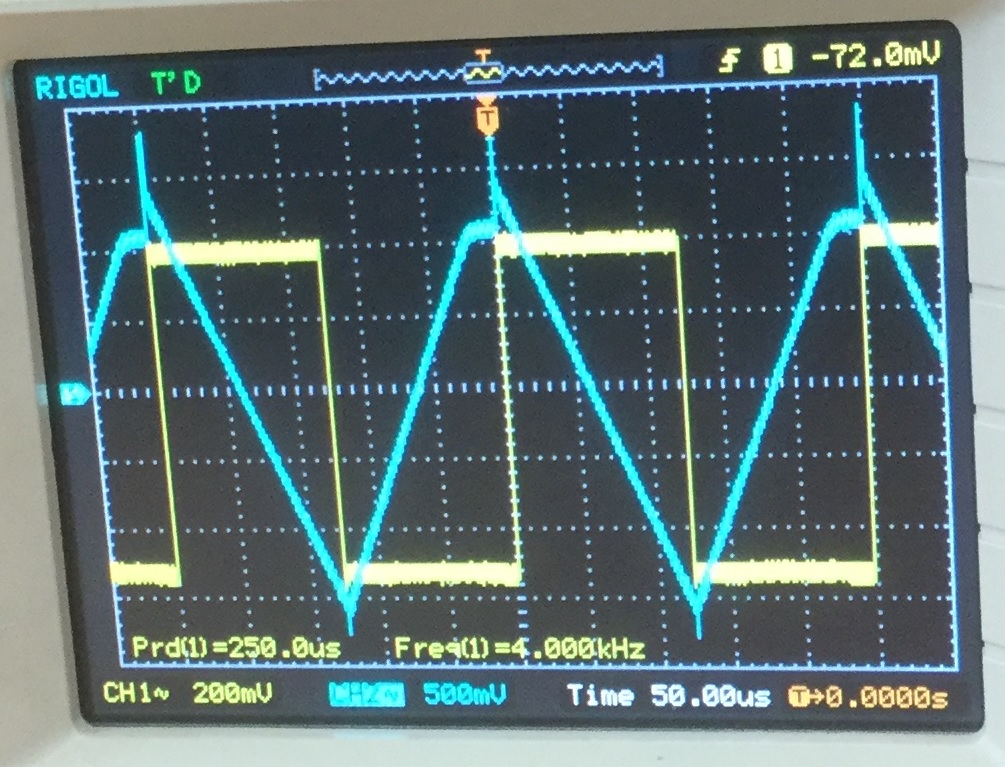
\includegraphics[scale=0.5]{r2c4}
\subsection*{6.}
tabelka?
\subsection*{7.}
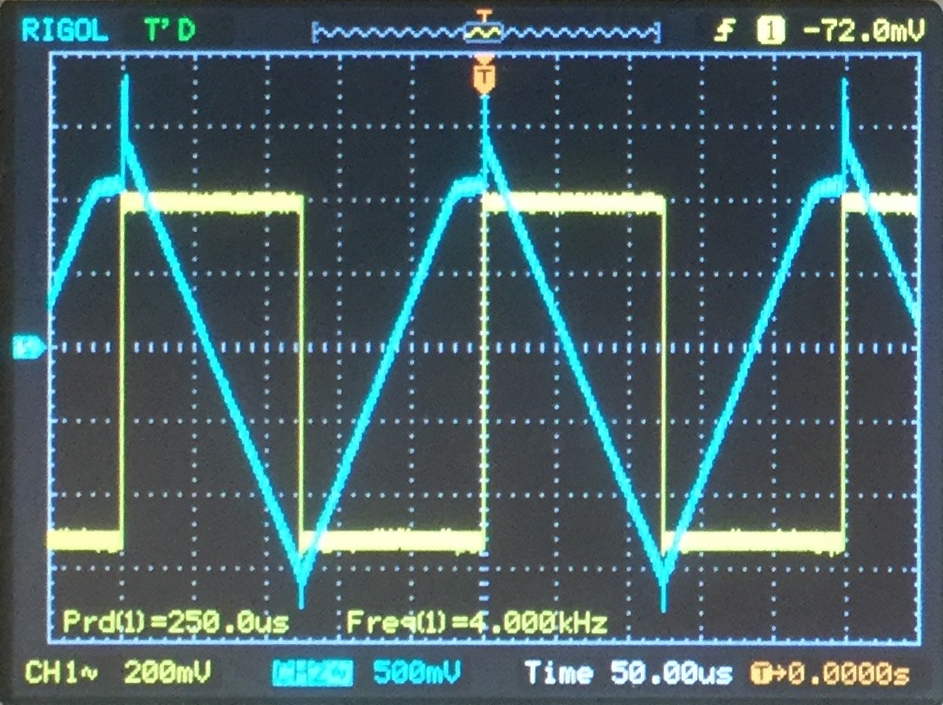
\includegraphics[scale=0.5]{czestotliwosc2}
\subsection*{8.}
Przykładowy oscylogram pary przebiegów:
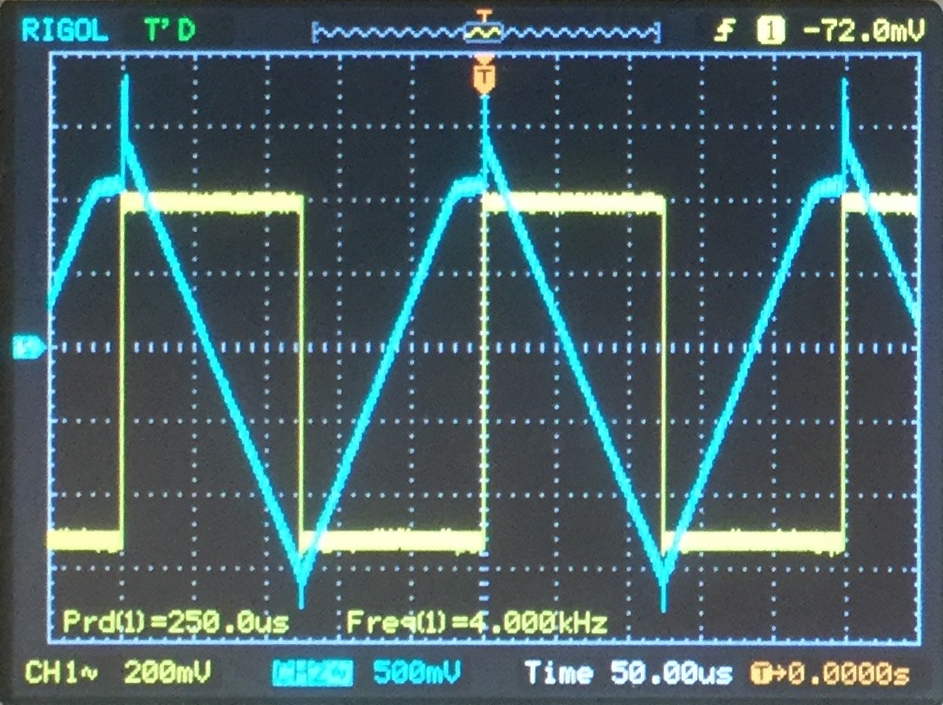
\includegraphics[scale=0.5]{czestotliwosc2}

\section{Zadanie 1.6}

\subsection*{1.}
schemat?
\subsection*{4.}
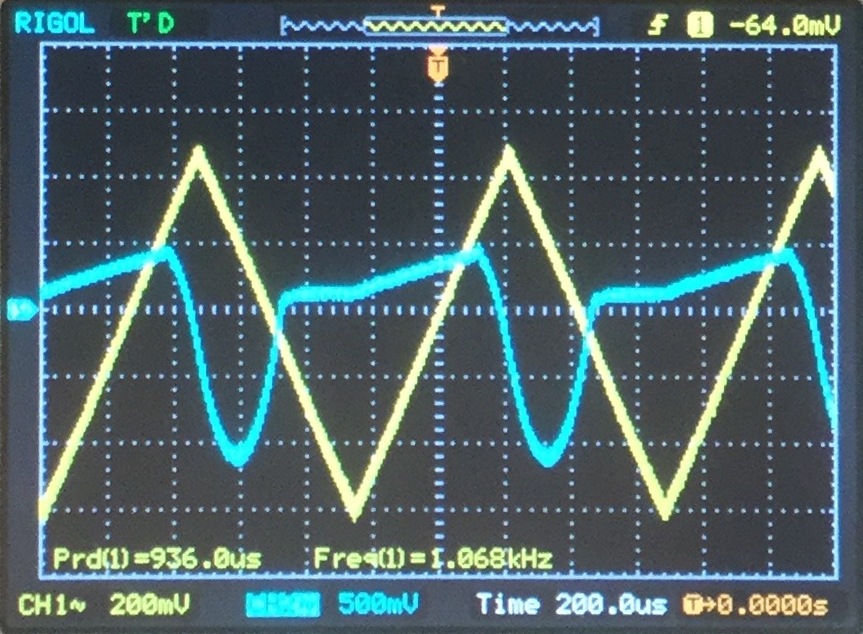
\includegraphics[scale=0.5]{czestotliwosc3}
\subsection*{5.}
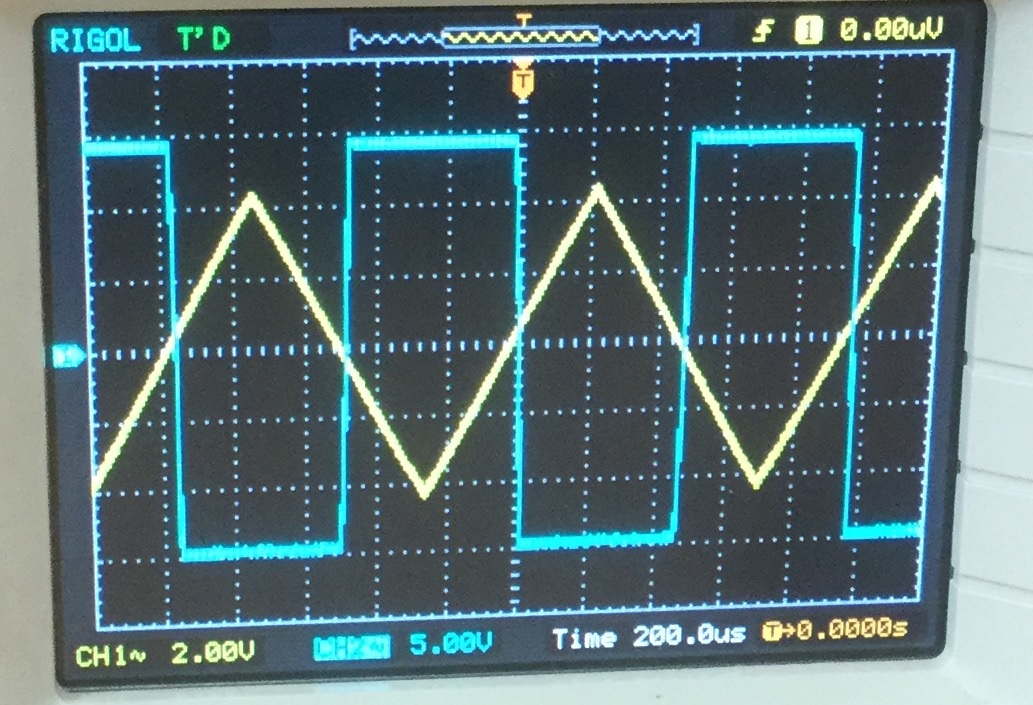
\includegraphics[scale=0.5]{przebieg_prostokatny}
\subsection*{6.}
Lepiej: 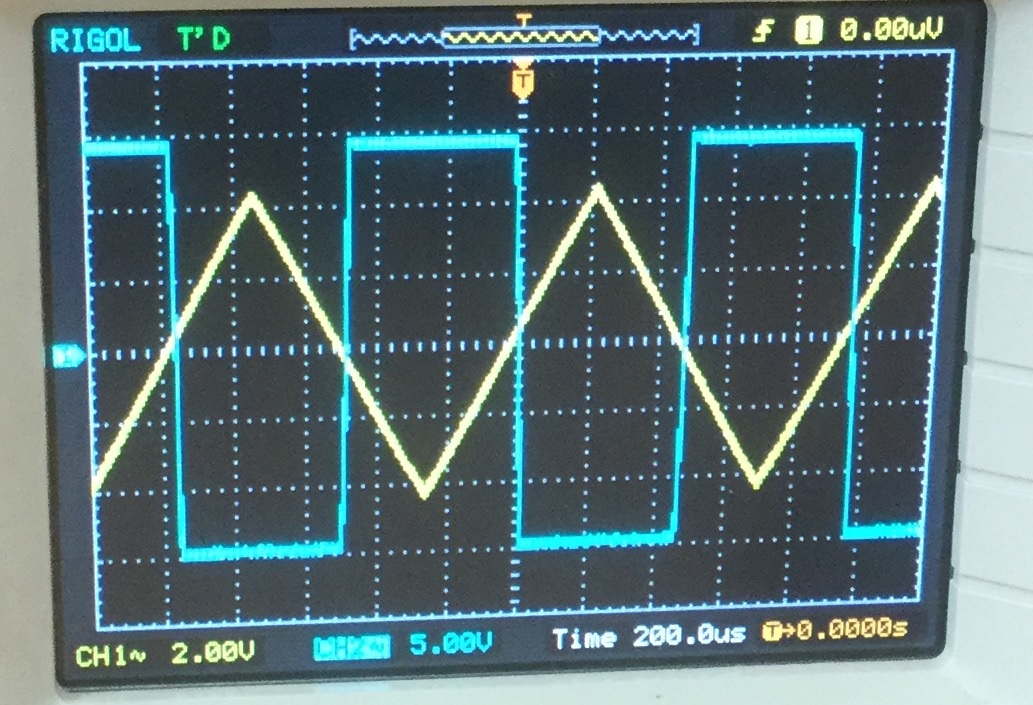
\includegraphics[scale=0.5]{przebieg_prostokatny}
Gorzej: 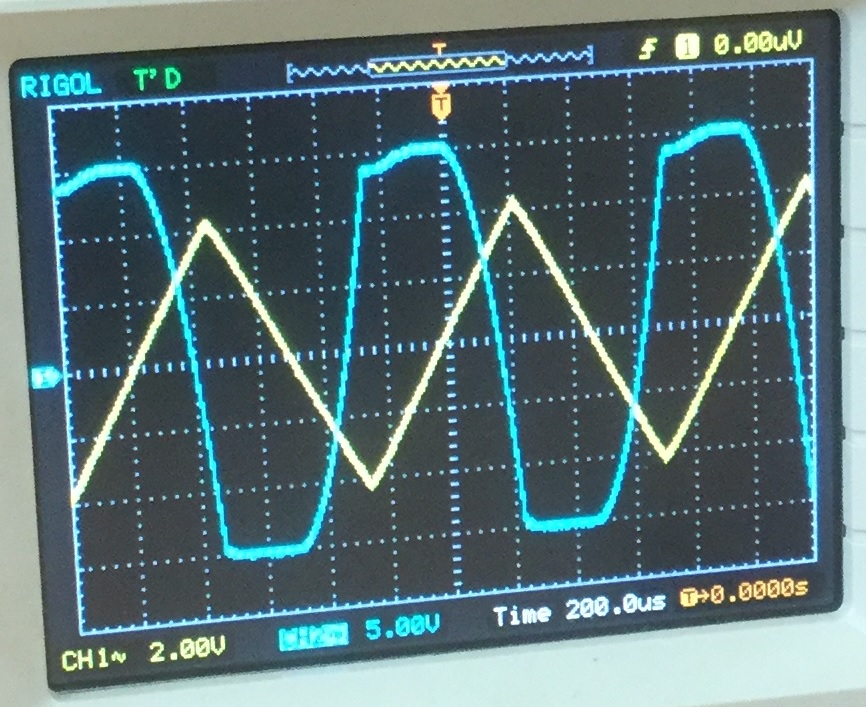
\includegraphics[scale=0.5]{gorzej}
\subsection*{7.}
wnioski


\bibliography{IEEEabrv,refs}

\begin{thebibliography}{9}

\bibitem{rlc}
  W trakcie przeprowadzania doświadczeń i pisania sprawozdania zespół korzystał głównie z materiałów ze strony http://mariusznaumowicz.ddns.net/materialy.html oraz z wiedzy własnej.\\


\end{thebibliography}

\end{document}7